
\chapter{KESIMPULAN DAN SARAN}

\section{Kesimpulan}
Berdasarkan hasil dan pembahasan terkait empat Model CNN dalam tugas "Prediksi Pose Semaphore," dapat diperoleh beberapa kesimpulan tentang kinerja masing-masing model. Selain kinerja masing-masing model juga dibahas tentang pengujian dilakukan dengan membandingkan performa Model CNN, Model CNN2, ResNet50V2, dan Xception dalam mengenali pose semaphore yang dihasilkan oleh sembilan koresponden berbeda dengan lima variasi gerakan dari huruf A hingga E. Berikut ini kesimpulan yang bisa diperoleh 

1. Perbandingan hasil loss dari keempat model (Model CNN, Model CNN2, ResNet50V2, dan Xception) pada Gambar \ref{fig:GrafikPerbandinganLoss} memberikan gambaran kuantitatif tentang performa dan konvergensi masing-masing model selama proses pelatihan. Semakin rendah nilai loss, semakin baik model tersebut dalam menemukan representasi yang tepat dari data dan mengoptimalkan parameter dalam rangka tugas pengenalan pose semaphore 

\begin{figure}[!hbt]
	\centering
	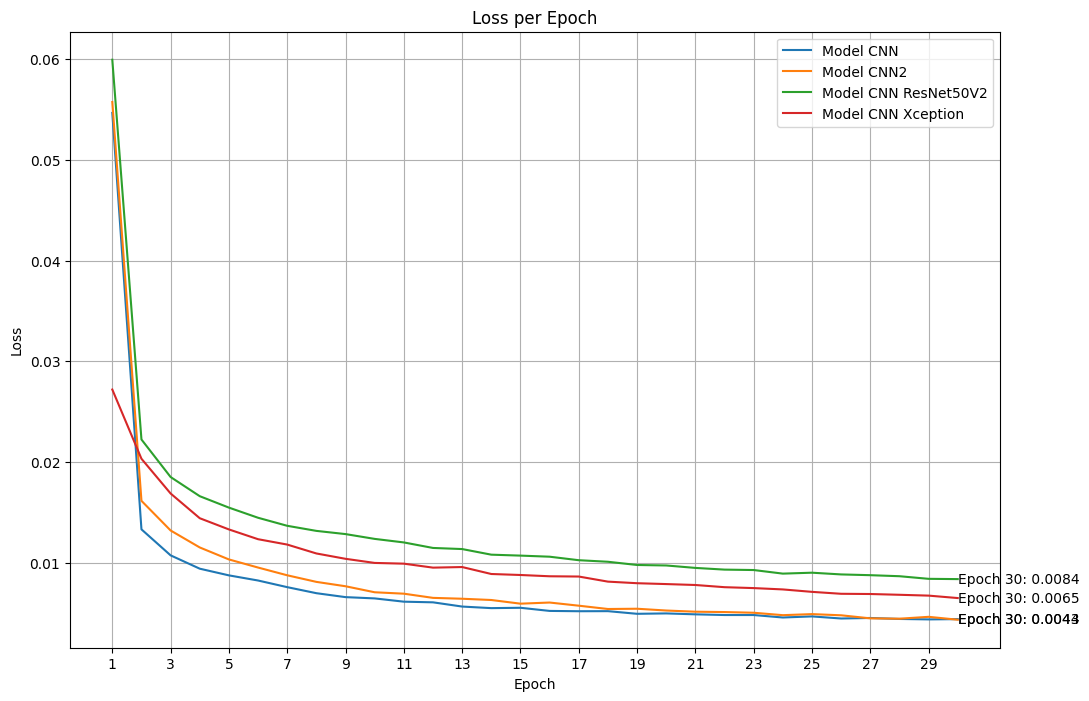
\includegraphics[width=0.7\linewidth]{gambar/bener/Perbandingan_LossCNN.png}
	\captionof{figure}{Grafik Perbandingan Loss}
	\label{fig:GrafikPerbandinganLoss}
\end{figure}

Model CNN dan Model CNN2 menunjukkan hasil yang lebih baik dibandingkan dengan ResNet50V2 dan Xception. Dari hasil loss yang terekam selama 30 \textit{epoch}, Model CNN dan Model CNN2 mencapai nilai loss terendah lebih cepat dan secara konsisten memiliki nilai loss yang lebih rendah dibandingkan dua model lainnya.

Model CNN mencapai nilai loss terendah sekitar 0.0044 pada \textit{epoch} ke-30, sedangkan Model CNN2 mencapai nilai loss terendah sekitar 0.0043 pada \textit{epoch} ke-29. Dalam kasus ini, Model CNN dan Model CNN2 memiliki hasil loss yang sangat mendekati satu sama lain, menandakan kualitas representasi yang serupa dalam tugas pengenalan pose semaphore.

Sementara itu, ResNet50V2 dan Xception juga menunjukkan penurunan nilai loss yang konsisten selama proses pelatihan. Namun, keduanya memiliki nilai loss yang agak lebih tinggi dibandingkan dua model sebelumnya. ResNet50V2 mencapai nilai loss terendah sekitar 0.0083 pada \textit{epoch} ke-30, sementara Xception mencapai nilai loss terendah sekitar 0.0065 pada \textit{epoch} ke-26.

2. Berdasarkan hasil perbandingan akurasi dari empat model sesuai dengan Gambar \ref{fig:GrafikPerbandinganAkurasi}, yaitu Model CNN, Model CNN2, ResNet50V2, dan Xception, pada \textit{epoch} terakhir yaitu epich ke-30 . terlihat bahwa Model CNN2 memiliki akurasi tertinggi pada epoch terakhir, yaitu sekitar 93.53\%. Model ini juga memiliki validasi akurasi yang cukup tinggi, mencapai sekitar 97.20\%. Model CNN mengalami performa yang hampir setara dengan Model CNN2, dengan akurasi pada epoch terakhir sekitar 93.72\%, dan validasi akurasi sekitar 97.50\%.

\begin{figure}[!hbt]
	\centering
	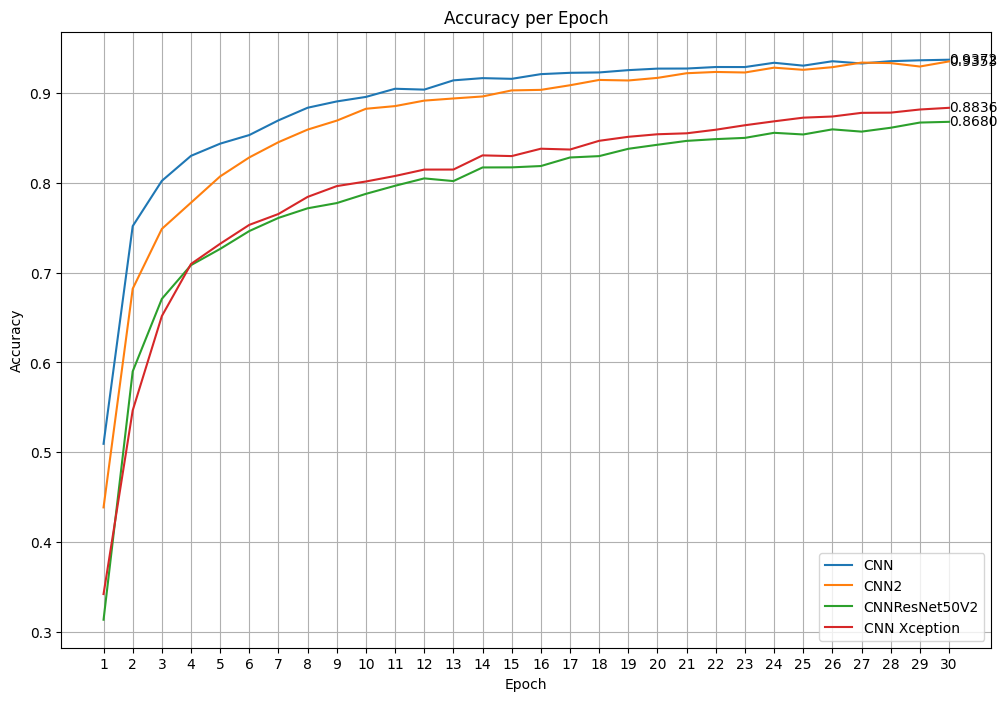
\includegraphics[width=0.7\linewidth]{gambar/bener/Perbandingan_AkurasiCNN.png}
	\captionof{figure}{Grafik Perbandingan Loss}
	\label{fig:GrafikPerbandinganAkurasi}
\end{figure}

Sementara itu, Model ResNet50V2 dan Model Xception memiliki akurasi yang sedikit lebih rendah daripada kedua model CNN tersebut. Model ResNet50V2 mencapai akurasi sekitar 88.36\%, dengan validasi akurasi sekitar 96.59\%. Sedangkan, Model Xception memiliki akurasi dan validasi akurasi yang sama dengan Model ResNet50V2, yaitu sekitar 88.36\% dan 92.39\% pada epoch terakhir.

Dari hasil ini, dapat disimpulkan bahwa Model CNN2 adalah yang memiliki akurasi tertinggi pada epoch terakhir, diikuti oleh Model CNN. Meskipun Model ResNet50V2 dan Model Xception memiliki akurasi yang lebih rendah, namun keduanya masih menunjukkan kinerja yang cukup baik dalam tugas klasifikasi pose semaphore.

\section{Saran}
Penelitian ini merupakan penelitian dasar yang dapat dikembangkan lebih lanjut diantaranya dengan  memperbanyak dataset huruf ,	Menambahkan variasi latar dan objek yang berbeda pada saat pengumpulan data , lebih teliti dalam memasukkan data pelatihan serta memperbaiki dalam kemampuan deteksi huruf